 \subsection{Anticipated total duration of the project}

The anticipated duration of the project is two years (24 months).

\vspace{-1em}
\subsection{Objectives}
\label{sec:objectives}

The objective of this project is to develop approaches that address the six key challenges raised in \autoref{sec:startingpoint}. As shown in \autoref{fig:approach}, the first three approaches will 
focus on \emph{data transformation}, jointly allowing us to automatically turn a UI log into an event log, through event annotation, noise removal, and case identification. The latter three approaches will focus on process representation, turning an event log into an appropriate process model, through  abstraction, labeling, and visualization.

\begin{figure}[h!]
	\centering
	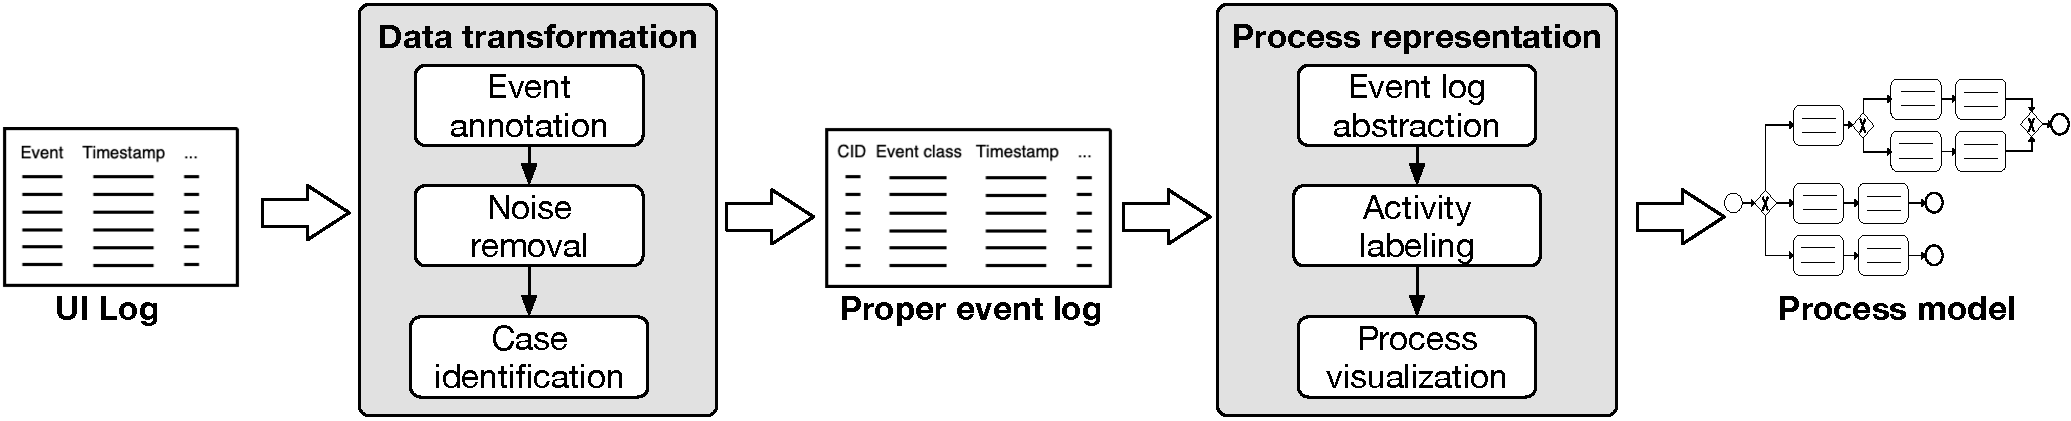
\includegraphics[width=\textwidth]{./figures/overview.pdf}
	\caption{Overview of the proposed project}
	\label{fig:approach}
\end{figure}

\subsection{Work programme including proposed research methods}
\label{sec:workprogramme}

\mypar{Package structure} In accordance with the outlined objectives, we divided the work programme into two work streams (WS1 and WS2), encompassing a total of six work packages (WP1 to WP6). Stream WS1, focusing on data transformation, will be led by the University of Mannheim and consists of WP1 to WP3. Stream WS2, targeting process representation, will be led by the Kühne Logistics University and consists of WP4 to WP6. We have designed the two work streams in such a way that they can be executed independently from each other. We achieved this by ensuring that WS2 can build on publicly available  UI logs until the first results from WS1 are available. Therefore, both work streams can immediately start in parallel. 

\mypar{Research method} We will achieve our objectives through the design, implementation, and evaluation of novel process mining approaches. Their implementation will be conducted in Python, based on the \textit{PM4Py} process mining library\footnote{\url{https://pm4py.fit.fraunhofer.de/}}. 
To evaluate the developed approaches, we will use publicly available real-world UI logs provided by the authors of \cite{leno2020identifying}\footnote{\url{https://figshare.com/articles/dataset/UI\_logs/12543587}}.
Should we identify a need for evaluation data beyond the publicly available logs, we will use the publicly available \textit{action logger}~\cite{leno2019action} tool to obtain additional UI logs. 
We will evaluate the approaches in WP1 to WP5 in terms of their \emph{accuracy} and \emph{efficiency}, e.g., with respect to manually established gold standards, whereas the \emph{usefulness} of the visualization approach developed in WP6 shall also be assessed through a user study. 

\vspace{-1em}
\subsubsection{WP1: UI log enrichment (7 PM)}
\label{sec:wp1}

Although events in UI logs can be associated with a broad range of relevant attributes, they fundamentally lack the \emph{event labels} that are required in process mining to indicate the meaning of events or to recognize equivalent ones (by using labels to define \emph{event classes}).
To illustrate this, consider the shortened version of our UI log in \autoref{fig:example_short}. 
In an event log with proper labels, event 1 would carry a label such as ``\textit{Receive order [via e-mail]}'', which would capture what exactly happened in the event (receiving an order) and, optionally, through which medium (e-mail).
However, instead of providing such process-relevant information, the UI log only explicitly captures that the event was a ``\textit{click}'' on a ``\textit{list}'' in the application ``\textit{Outlook}''. 

% That this click relates to receiving an order from a customer can only be inferred from the associated e-mail. 
% Events 4 and 14 also highlight the importance of proper event labels for classifying events. Looking at the values of the key \textit{Event}, \textit{Application}, \textit{Element label}, and \textit{Element type} attributes, they appear to be identical. However, they occur in different applications (Salesforce and Facebook, respectively), and, furthermore, event 4 leads the user to a log-in screen (password entry succeeds the event), while event 14 completes the log-in process (password entry precedes the event). Proper labels would clarify such differences, ensuring that events 4 and 14 are recognized as distinct process steps.

% The problem is that this labeling task is complex in reality. For example, only the \textit{URL} attribute helps to recognize that the specific application context differs between events 4 and 14.
% In contrast, it may also be hard to recognize that certain events actually do relate to a similar context. For instance, events 4 and 7 both relate to activities in Salesforce, though their URLs differ considerably. At other times, as seen for event 1, labeling information needs to be derived from free-text attribute values, such as the contents of a message.

% For example, consider events 4, 7, and 13. According to the UI log, these events all occurred in the context of the application ``\textit{Chrome}'', i.e., an Internet browser. However, a brief analysis of the respective URL attributes reveals that event 4 relates to Salesforce and event 13 relates to Facebook. The fact that event 7 also relates to Salesforce is actually hard to identify since the URL structure of Salesforce changes once the user has logged into the application. 

\begin{figure}[h!]
	\centering
	\begin{adjustbox}{max width=\textwidth}
		\begin{tabular}{llllllll}
			\hline\noalign{\smallskip}\noalign{\smallskip}
			\textbf{ID} &\textbf{Timestamp}&\textbf{Event}&\textbf{Application}&\textbf{Element label}&\textbf{Element type}&\textbf{Element value}&\textbf{URL}\\
			\noalign{\smallskip}\hline\noalign{\smallskip}
			1&08:35.2&click&Outlook&Customer X - O123&list&Please initiate an order …&-\\\noalign{\smallskip}
			...&...&...&...&...&...&...&...\\
			4&08:39.7&click&Chrome&Log in&button&-&https://www.salesforce.com/\\\noalign{\smallskip}
			5&08:40.0&change&Chrome&Password&text field&-&https://login.salesforce.com/\\\noalign{\smallskip}
			6&08:40.5&click&Chrome&Submit&button&-&https://login.salesforce.com/\\\noalign{\smallskip}
			7&08:52.6&click&Chrome&New Account&button&-&https://com.lightning.force.com/home\\\noalign{\smallskip}
			...&...&...&...&...&...&...&...\\
			13&08:40.0&change&Chrome&Password&text field&-&https://www.facebook.com/\\\noalign{\smallskip}
			14&08:42.9&click&Chrome&Log in&button&-&https://www.facebook.com/\\\noalign{\smallskip}
			15&08:42.9&click&Chrome&Messenger&button&-&https://www.facebook.com/\\\noalign{\smallskip}
			...&...&...&...&...&...&...&...\\
			\hline\noalign{\smallskip}
		\end{tabular}
	\end{adjustbox}
	\caption{Shortened version of UI log from \autoref{fig:example}}
	\label{fig:example_short}
\end{figure}


\mypar{Approach overview}
To overcome this limitation in UI log data, this work package sets out to develop an approach for the semantic annotation of UI events. Specifically, our approach will enrich raw event data with dedicated attributes that capture
 \textit{which action} was applied to \textit{which object} and in \textit{which context}. The former two aspects are common components of activity and event labels~\cite{mendling2010activity,leopold2019using}, whereas the context (e.g., ``\textit{via e-mail}'' or ``\textit{in Salesforce}'') is incorporated because UI logs often span multiple applications, allowing us to distinguish events that appear to be similar, but occur in distinct parts of a process. 
 Our approach will achieve this in two steps:


\mypar{Step 1: Action and object identification} Our approach will use different strategies to identify the action and object to which an event applies. The proposed strategies differentiate between \textit{button click},  \textit{data entry}, and \textit{data receipt} events, tailored to their structural differences:
%
\mypartwo{Button click events}  For events corresponding to a user clicking on a button, we will analyze the textual information associated with that button (typically the button's label, e.g., ``\textit{Submit}'', ``\textit{New Account}''), or ``\textit{Upload files}''. To do this, we will use a fine-tuned BERT~\cite{Devlin2019} model to tag the tokens in a given text as relating to an action (\texttt{ACT}), a business object (\texttt{BO}), or a miscellaneous class (\texttt{X}), obtaining, e.g., \textit{submit}\textbackslash\texttt{ACT}, \textit{new}\textbackslash\texttt{BO} \textit{account}\textbackslash\texttt{BO}, and \textit{upload}\textbackslash\texttt{ACT} \textit{files}\textbackslash\texttt{BO}.
Finally, to ensure that each event is associated with an action, if no \texttt{ACT} tag is assigned, we will associate the event with an action from a repository of standard actions (e.g., \textit{create} or \textit{modify}). To do this, we will use a recently developed classifier~\cite{rebmann2022enabling} that determines the most suitable action type based on the available textual information. For instance, ``\textit{new account}'' best corresponds to a \textit{create} action, which means that for event 7 our approach will return \textit{action: ``create''}, \textit{object: ``new account''}.
%
\mypartwo{Data entry events} Data entry events correspond to events that set or change a value, e.g., in a free-text field, a drop-down menu, or a radio button. Our approach will use the information from the elemental label (e.g., ``\textit{Password}'', ``\textit{order amount}'', or ``customer type''), if available, or otherwise the value that is set from a drop-down menu (e.g., ``premium customer''). Given such a text, we will use the same tagging model as for button clicks to identify actions and objects. Afterwards, if no action was identified, we  set the associated action to \textit{enter}, \textit{select}, or \textit{set} depending on the element type, e.g., yielding 
\textit{action: ``enter''}, \textit{object: ``password''} or \textit{action: ``select''}, \textit{object: ``customer type''}.
%
\mypartwo{Data receipt events} Finally, data receipt events correspond to any event that is about receiving or reading free-text information, such as opening an e-mail or reading a message. These events are the most challenging to annotate, given that an e-mail or message can relate to virtually any topic.
To handle this diversity, our approach will first process the opened text using a recently proposed transformed-based approach for \textit{e-mail intent mapping}~\cite{Khandaker2022transformer}, which will turn a larger message into a single phrase such as ``\textit{a meeting is being proposed}'' or ``\textit{an order is being placed}''. Next, we will use a fine-tuned BERT model to transform this phrase into a single object and adding a \textit{receive} or \textit{open} action, e.g., turning  ``\textit{a meeting is being proposed}'' into \textit{action: ``receive''}, \textit{object: ``meeting proposal''}.

\mypar{Step 2: Context identification} Next, our approach identifies the specific application or sub application in which an event is performed, adding it as a \textit{context} attribute to the event. 
For events performed by interacting with non-web applications, we directly derive the context based on the \textit{application} attribute associated with an event.
For browser-based events, instead, we set the context as the specific web application that an event relates to. To identify this, our approach will first apply string matching on the event's URL. For instance, 
after removing URL-specific prefixes and suffixes from event 4 in \autoref{fig:example_short}, we obtain ``\textit{salesforce}'', which can be easily verified as a business application using public resources. 
For events where this strategy does not deliver a conclusive result, we then turn to the event's broader context. For example, for event 7, the string matching strategy is unlikely to deduce that this event occurred in Salesforce. However, when taking the log's context into account, we can clearly identify a number of sub applications, such as Salesforce (from event 4) and Facebook (from event 13). Although the URL of event 7 is rather cryptic, comparing it against the two available options will clearly identify Salesforce as the most likely sub application. In this way, we enrich the UI log with the specific application in which each event occurred, enabling context-aware analysis of events in downstream tasks.


\subsubsection{WP2:  Noise removal (7 PM)}
\label{sec:wp2}

UI logs often contain events that do not relate to the business process under investigation, such as events related to private activities (e.g., checking Facebook) or to non-related business activities (e.g., filing a reimbursement form of a business trip).
Given that process mining techniques assume that the events in a log relate to a single process, these irrelevant events, also referred to as \emph{noise}, need to be identified and removed from a UI log.

While various noise detection techniques already exist (cf., \autoref{sec:stateoftheart}), these  inherently approach noise detection from a different angle. Particularly, they aim to detect process behavior that stands out in terms of frequency (such as rare occurrence of an order being accepted before it is created), i.e., they try to \emph{detect events that are behavioral anomalies}, e.g., caused by recording errors.
When dealing with UI logs, we need to \emph{detect events that do not relate to the process at hand}. 

\mypar{Approach overview}
To tackle this task, we propose to develop a semantic noise detection approach tailored to the specifics of UI logs. Our approach will capture noise detection in the form of a classification task, aiming to classify events as \emph{process relevant} or not, based on the textual contents of their attributes. We will develop and compare several classifiers, to determine the best way to operationalize our approach. Specifically, we will test a traditional machine learning model using feature embeddings and standard classifiers, as well as a deep learning model using transformers.

\mypar{Model 1: Embedding-based classification}
We will assess the potential of traditional machine learning by first transforming the textual input data associated with an event into a high-dimensional feature vector using \textit{embedding} techniques. In this manner, we encode both general event information in features, as well as process-specific information extracted in the previous step, i.e., the event's action, business object, and application. We will obtain (and compare) embeddings using established methods, such as through GloVe embeddings~\cite{pennington2014glove} and SentenceBERT~\cite{reimers-2019-sentence-bert}.
\newline 
Given such embeddings, noise identification can be approached  using standard classifiers, for which we expect support vector machines (SVMs) to be well-suited. 
We will test and compare single-class and two-class classification strategies for this.
Single-class classification involves training a classifier that recognizes which events are related to a specific process by assuming that the majority of events in a UI log are related to that. While such an approach thus would not require any user input, the classification accuracy may be improved in a two-class setting, where users explicitly label some events as process relevant and irrelevant (i.e., ground-truth labels). 

\mypar{Model 2: Transformer-based classification} 
Aside from traditional machine learning techniques, we will also test state-of-the-art transformer-based models to classify events as noisy or not. We will achieve this by fine-tuning a transformer, such as BERT~\cite{Devlin2019}, directly on the text-classification task at hand. 
Again, we will test both single-class and two-class scenarios here.
\newline Although the potential of such transformers is well-known, it will be interesting to see how well they perform in comparison to embedding-based models in situations with relatively small amounts of training data, which is important in the context of UI log analysis.

Depending on the outcome of our experiments, our final approach will either consist of one specific classification technique, or will provide recommendations on which technique to use in a given situation, e.g., depending on the size of the UI logs and the availability of ground-truth labels.


% \mypar{Outcome}
% The outcome of this work package is a classification approach that identifies irrelevant events in a UI log. Depending on the outcome of our experiments, the approach will either consist of one specific classification technique, or will involve a recommendation on which technique to use in what situation, e.g., depending on the size of the UI logs and the availability of ground-truth labels.
% The approach will be applicable without requiring any additional user input, though users may improve the approach's accuracy by providing manually classified events or process-specific artifacts (e.g., a process model) as input.

\subsubsection{WP3: Case identification (10 PM)}
\label{sec:wp3}

Once irrelevant events have been filtered out from  a UI log, we next need to recognize which events belong to the same process instance, e.g., to the same customer order or service ticket, a task referred to as \emph{case identification}.

Existing techniques that address this task in general process mining settings primarily base the identification on co-occurrence statistics, which reveal behavioral regulations in an event log (cf., \autoref{sec:stateoftheart}). Such techniques work well for relatively structured settings, 
but they are not sufficient when dealing with event data stemming from more flexible environments, in which the execution of several cases overlap. This is, e.g., seen in the example of \autoref{fig:example}, where the first three events each start a new process instance, by initiating three different orders in a batch-like manner. This, therefore, calls for a new case-identification approach, tailored to the specifics of the UI logs.

\mypar{Approach overview}
This work package sets out to develop such a new approach for case identification in UI logs, which we achieve by tackling it as a \textit{matching problem}.
Following established practice in this regard~\cite{gal2011uncertain}, our approach will start by applying \textit{first-line matchers} on the events in a UI log, which compute similarity scores between pairs of events, and then apply a \textit{second-line matcher} that uses these computed similarity scores to find an optimal overall alignment among the events in a UI log. The resulting alignment will capture  which events belong to each other, i.e., which are determined to be part of the same case.

\mypar{Step 1: First-line matching} 
We will establish different first-line matchers, each dedicated to quantifying the similarity between two events from a particular perspective. Particularly, we will include matchers that consider:  1) \textit{Behavioral relatedness}, 
which can recognize events that are observed to commonly co-occur or follow each other, similar to techniques used to capture behavioral regularities in event logs~\cite{diba2020extraction,ferreira2009discovering} and those proposed in the context of task mining on structured UI logs~\cite{leno2020identifying,Urabe21}.
2) \textit{Semantic relatedness} between events, e.g., to  recognize that an order cannot be \textit{accepted before it is created}, which means that events appearing in that order cannot belong to the same case, for which we will exploit semantic regularities captured in our earlier work~\cite{van2021natural}. 3) \textit{Shared identifiers}, which will look for mentions of specific identifiers (e.g., ``Customer X'' or ``O123'') that can be helpful to recognize events that relate to the same object, when such information is available. 


\mypar{Step 2: Second-line matching} Having obtained multiple sets of similarity scores over the event-pairs in a UI log, our approach will then use these scores, in combination with relevant cardinality constraints (e.g., each event belongs to exactly or at most one case) to establish an optimization problem. We will represent and solve these problems using Markov logic networks~\cite{lowd2007efficient,richardson2006markov}, which we have successfully used to solve other matching problems before~\cite{leopold2015towards}.
In this manner, our approach will obtain an event grouping that maximizes the different kinds of similarity (according to learned parameter weights) in light of the applied constraints, thus yielding groups of events that are determined to belong to the same case.

In this manner, the transformation from a UI log into an event log suitable for process mining is complete.

%
%
%Specifically, to determine the likelihood that events belong to the same case from a semantic viewpoint, e.g., because both refer to a same order ID or mention the same customer name, we frame the comparison of the events as an \emph{instance-based schema matching} task. For this, we recognize that events stemming from a particular application can be represented as instances in a particular schema (characterized by their payload attributes), enabling the application of existing matching techniques (cf., \cite{rinaldi2018matching,lehmberg2017stitching}).
%
%\mypar{Optimization} Having obtained similarity scores between individual events, these scores can then be used together with behavioral regularities identified by existing techniques~\cite{diba2020extraction,ferreira2009discovering} and cardinality constraints (e.g., each event belongs to exactly or at most one case) to establish an optimization problem, specifically using a Markov logic network. By solving this problem, we will obtain an event grouping that maximizes the semantic similarity and respects the identified behavioral regularities for each of the identified cases.

% % \mypar{Outcome}
% % The outcome of this work package is a case-identification approach that groups together events belonging to the same case, so that each case consists of a sequence of events that relate to the same process instance.
%  This completes the transformation from a UI log into an event log suitable for process mining.


\subsubsection{WP4: Event abstraction (6 PM)}
\label{sec:wp4}

\begin{wrapfigure}{r}{0.5\textwidth} 
	\vspace{-25pt}
	\begin{center}
		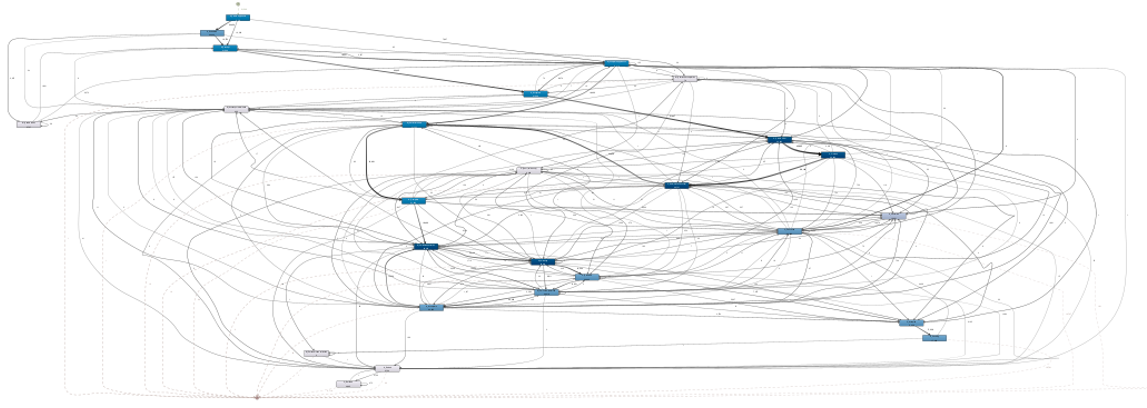
\includegraphics[width=\linewidth]{./figures/spaghettiprocess.png}
		\caption{A so-called spaghetti process model}
		\label{fig:spaghetti}
	\end{center}
	\vspace{-15pt}
	\vspace{1pt}
\end{wrapfigure} 
Even after transformation into a proper event log, the logs stemming from UI recordings comprise low-level event data, in which each event corresponds to a small action performed by a user. This fine-granular nature makes the data unsuitable for meaningful process analysis since the application of discovery techniques yields so-called \emph{spaghetti models}, as e.g., depicted in \autoref{fig:spaghetti}. To tackle this issue, various techniques for grouping low-level events into high-level activities have been defined (see \autoref{sec:stateoftheart}). However, these approaches do not allow to define \emph{what properties} the abstracted log shall satisfy. Hence, it is hard to ensure that the resulting abstraction is appropriate for a specific analysis goal. 

%this purpose exist. Yet, their focus is on \emph{how} the abstraction is conducted, rather than \emph{what properties} the abstracted log shall satisfy. Without dedicated control on the result of event abstraction, however, it is hard to ensure that an abstraction is appropriate for a particular context or specific analysis goal. 
%To tackle this issue, event abstraction is a commonly used means to lift the event sequences of a log to a more abstract representation, by grouping low-level events into high-level activities. 

\mypar{Approach overview}
To overcome this limitation, we will develop an approach for \emph{constraint-driven event abstraction}. Based on 1) a number of distance functions that quantify the similarity between events and 2) a set of (user-defined) constraints, our approach identifies an optimal log abstraction using \textit{constraint-based clustering}. That is, it groups together low-level event classes into high-level activities such that the abstracted log is meaningful for downstream analysis. The outcome of our approach, therefore, is an event log with respective high-level activities that provides clear insights into the high-level process behavior contained in the UI log.

%This is particularly problematic in the context of UI logs, since these have clear characteristics that should or can be exploited to guide the abstraction task.
%\mypar{Constraint-driven event abstraction}
\mypar{Step 1: Distance computation} First, we need to determine which low-level event classes are similar to each other. Note that this is conceptually comparable to step 1 from WP3, where we identify which events belong to the same case. While some ideas from WP3 can be applied here as well, there is a need to identify groups on lower level of granularity and with a particular focus on cross-case behavior. To this end, we define three different \textit{distance functions}: 
1) We use a temporal distance function $d_{tmp}$ to quantify how much time passes typically between instances of two event classes. Intuitively, event classes belonging to the same group should also commonly occur shortly after each other. 
2) We will use a behavioral distance function $d_{bhv}$ to quantify the correlation of event classes from a control-flow perspective.
% strength of the order relationship between two event classes. Given classes $c_1$ and $c_2$, the distance function $d_{bhv}$ captures how often we observe events of $c_1$ before those of $c_2$ or the other way around. 
As explained in WP3, there are different ways to detect and quantify this and we will build on existing work from behavioral analysis~\cite{diba2020extraction,ferreira2009discovering} and task mining~\cite{leno2020identifying,Urabe21} to operationalize this.  
3) We use a semantic distance function $d_{sem}$ to quantify to what extent two event classes are concerned with the same task. To capture this, we will leverage available information about the event context, such as the application in which the event is executed or the data that is entered or processed during the event execution. 

\mypar{Step 2: Constraint generation} Second, we need to determine which constraints need to hold in order to obtain a meaningful event abstraction. An obvious and simple solution is to ask the user for input on that matter. However, while such user-defined constraints can lead to meaningful event abstraction, it may not always be obvious to users which constraints they shall request. Therefore, we will develop an algorithm that suggests potential constraints on the event data. To this end, we will identify which attribute values  lead to a clear separation between different groups of event classes from a control-flow or temporal perspective, e.g., by considering aspects such as cohesion and coupling over the  abstracted log~\cite{vanderfeesten2007quality}. A prime challenge here will be to obtain suggestions in a computationally efficient manner, given the high dimensionality of the task. We aim to deal with this by reducing the problem size through decomposition of the event data, e.g., on the directly-follows graph, and by considering the characteristics of data attributes in the log, e.g., through data profiling~\cite{papenbrock2015data}, allowing us to discard unpromising attributes in advance.

%While our approach shall support a broad range of constraint types, common ones to impose in the context of UI logs are, for instance, constraints that ensure that each high-level activity only comprises events that stem from the same application (to ensure semantic cohesion) or occurred within a certain timespan of each other (to ensure behavioral cohesion). 

\mypar{Step 3: Constraint-based Clustering} Third, we use the output from the distance computations from step 1 and the set of constraints from step 2 to determine the final 
clusters of event classes, which can then be used to abstract the cases in the event log. Intuitively, the distances determined via the three distance functions should be minimized, while still meeting the imposed constraints. To implement this, we will build on an existing approach for clustering with instance-level constraints~\cite{wagstaff2000clustering}. 


%\mypar{Solution algorithms}
%To guarantee an optimal solution, we will initially develop an approach for exhaustive log abstraction. Yet, striving for more efficient processing, we will also provide a heuristic version that is guided by behavioral dependencies found in the log, e.g., by recognizing certain event classes that shall never be grouped into a single activity due to their relative positions in traces. As such, this heuristic version shall aim to considerably improve the computation time, with limited impact on the quality of the obtained results.


%\mypar{Outcome} The outcome of this work package is an approach that allows users to abstract a low-level event log into high-level activities based on generated or user-defined abstraction requirements, providing clear insights into the high-level process behavior contained in the UI log.

\subsubsection{WP5: Activity labeling (8 PM)}
\label{sec:wp5}

The value of a discovered process model highly depends on the quality of its activity labels, since these labels form the basis of what a human can understand about the process~\cite{mendling2010activity}. Recognizing this,  the importance of clear and informative labels in process models has led to a large body of literature concerned with labeling guidelines~\cite{mendling2010seven,leopold2015learning} and their automatic enforcement~\cite{leopold2013detection,becker2009towards}. 
These best practices indicate that process model activity labels should contain an action provided as an imperative verb (e.g. ``\textit{create}" or ``\textit{send}'') and at least one business object provided as a noun (e.g. ``\textit{order}'' or ``\textit{e-mail}''). Additional information can be provided at the end of the label if required. Following these rules results in labels such as ``\textit{Create order}'' or ``\textit{Send e-mail to customer}''. 

The challenge in the context of this work package is to automatically generate meaningful labels for each group of UI events that has been identified in the event-abstraction step (WP4). To illustrate this, consider the events 4, 5, and 6 from the UI log in \autoref{fig:example}, which, respectively, refer to the pressing of a log-in button, entering a password, and pressing the submit button.
Recognizing the joint role of these events in the process, a proper label for the group could be ``\textit{Log into Salesforce}", which summarizes both the outcome (logging in) and the context (Salesforce) of the event group. 
However, automatically generating such \textit{higher-level labels} is complex, since it requires to infer an overarching activity from the actions, business objects, and application contexts of multiple low-level events. Furthermore, how to derive such an overarching label depends on the nature of the events and, thus, differs per situation. 

\mypar{Approach overview}
In light of these challenges, we propose a novel activity labeling approach. In a first step, our approach uses three different strategies to generate different \textit{label candidates}. The rationale behind having different strategies is that a considered group of UI events can be described in different ways. In a second step, our approach then selects the most suitable labeling strategy based on behavioral and semantic analysis of the considered UI events. The outcome of our approach, therefore, is a higher-level activity label for a given set of UI events.  These labels are then used as additional annotations for the log stemming from WP4, resulting in an abstracted and meaningful event log. 

\mypar{Step 1: Label candidate generation} To generate higher-level labels, we jointly analyze the behavioral and semantic perspectives of grouped events. Building on observations from earlier work on process model name generation~\cite{leopold2014simplifying}, we define three specific strategies to generate label candidates: 
%
\mypartwo{Outcome-oriented labeling}
This strategy builds on the observation that a \textit{result} of a set of UI events can be used to describe the previous steps.  
 As an example, consider the ``\textit{Log into Salesforce}" label for events 4, 5, and 6. In line with earlier work, we  will derive such outcome-oriented labels by using the low-level labels from the first or the last event of a considered UI event group~\cite{leopold2014simplifying}.  
%
\mypartwo{Decision-based labeling} This strategy will exploit the fact that many processes are driven by key decisions, such as rejecting or accepting an offer from a customer. If a considered group of events encompasses such a decision point, we extract the main object that is affected by the decision and capture it in a high-level label, such as ``\textit{Decide about customer offer}''. 
%
\mypartwo{Holonym-based labeling}
This final strategy considers a setting where low-level events jointly contribute to a higher-level activity. In linguistics, a \textit{holonym} is a term that has a part-of relation with a number of \textit{meronyms}, e.g., a ``\textit{finger}'' is a meronym of the holonym ``\textit{hand}''.
By applying the notion of holonymy to events, we aim to recognize actions or business objects that are considered to be meronyms, allowing us to detect the holonym describing the higher-level activity. As an example, consider events 11, 12, and 13 from \autoref{fig:example}. While these events are essentially copy and paste operations, they all contribute to a higher-level event that could be described as ``\textit{Create customer account in Salesforce}''. To detect such holonym relations, we will leverage techniques from ontology learning~\cite{al2020automatic,wong2012ontology}. In this way, we overcome the limitations of previous work ~\cite{leopold2014simplifying} which built on the lexical database WordNet and, hence, was limited with respect to the scope.   

%We shall turn each of these strategies into an automated label-generation technique. This involves dealing with specific challenges caused by the process-specific nature of the data our project deals with. For example, with respect to the latter strategy, existing work has tried to address the problem of holonymy detection on process model activities by building on WordNet~\cite{leopold2014simplifying}. Yet, while WordNet is useful to detect general-purpose holonymy relations (such as between ``\textit{finger}'' and ``\textit{hand}''), it fails to detect more complex and domain-specific relations commonly found in process-mining contexts. Therefore, we will leverage techniques from ontology learning~\cite{al2020automatic,wong2012ontology} to automatically derive holonymy relations from general and domain-specific text corpora.    

\mypar{Step 2: Strategy selection} The three strategies  result in different labels for the same group of events. Therefore, the second step is to select the most appropriate labeling strategy. To this end, we again build on a  behavioral and semantic analysis of the low-level events involved and implement respective selection rules.  We pick outcome-oriented strategy if the group of events represents a synchronization point in a process, such as a \emph{log-in step}, which is succeeded by various other paths. We pick the decision-based strategy if the behavioral relations indicate a choice in the process as signaled by mutually exclusive events or when low-level actions have clearly opposite meanings, e.g., \emph{reject} versus \emph{accept}. Finally, we pick the holonym-based strategy when holonym relations can actually be identified for the given low-level events. In unclear cases, we stick to the first strategy as this will always deliver a result.  

%\mypar{Outcome} 

\subsubsection{WP6: Visualization (10 PM)}
\label{sec:wp6}

The final step is concerned with the visualization of the process captured in the UI log. In traditional process discovery, this is achieved by generating respective process models. Depending on the employed discovery algorithm, the resulting process model could be a Petri net \cite{van2004workflow}, a BPMN model \cite{conforti2016bpmn}, or a process tree \cite{leemans2013discovering}. While each algorithm and output representation comes with advantages and disadvantages, there is no specific discovery technique available tailored to the kind of UI-based event logs resulting from WP1 to WP5. %for the UI log generated in WP1 to WP5. 
The specific challenge is that the original level of granularity of the UI log is not appropriate for visualization since the number of events is too high. Yet, the user might be interested in getting insights into this level to fully understand how the process is executed. What is required is a dedicated \textit{visualization approach} that allows the user to adapt the process visualization in a flexible manner with respect to 1) the abstraction level and 2) the general scope. In the context of data warehousing and OLAP \cite{chaudhuri1997overview}, the former corresponds to \textit{drilling down} and \textit{rolling up}, while the latter corresponds to \textit{slicing}. 

\mypar{Approach overview}
In line with the requirements outlined above, we will propose a novel interactive visualization approach that allows the user to adapt both the abstraction level and the scope of the discovered model. To adapt the abstraction level, we introduce a \textit{slider-based} mechanism that allows the user to drill down or roll up. To adapt the scope, we introduce a \textit{semantic scoping} mechanism which provides the user with the possibility to limit the scope with respect to certain objects or applications. The outcome, therefore, is a novel discovery and representation approach that can visualize UI logs in a flexible fashion. As such, it completes our overall pipeline for semantic process discovery from UI logs. 

\mypar{Slider-based abstraction} The general idea of adapting the level of abstraction using a slider approach is present in several commercial process mining tools, such as Celonis\footnote{\url{www.celonis.com}} and Disco\footnote{\url{https://fluxicon.com/disco/}}. However, they implement abstraction by removing arcs or nodes based on their frequency. Our idea is to merge events based on the abstraction mechanism introduced in WP4 and use the approach from WP5 to present meaningful labels to the user. In case the user is interested in more details, they can drill down on individual events or groups thereof and explore the process on several levels at the same time. To this end, we will build on the ideas on multi-level discovery from \cite{leemans2020using} and adapt them to the specific scenario of slider-based abstraction. 

\mypar{Semantic scoping} Besides adapting the level of abstraction, the user might also want to modify the general scope of the discovered model. It is well imaginable that, for instance, there are specific applications or business objects in the process the user wishes to investigate further or, in the opposite case, remove them from the visualization. We, therefore, introduce a scoping  mechanism that allows the user to select applications and business objects that should be included or removed. To accomplish this, we employ a fine-tuned version of the open-source language model BLOOM \cite{scao2022bloom}. More specifically, we fine-tune BLOOM with a number of UI log traces such that BLOOM can learn about both semantic and behavioral aspects of typical UI events. Using the fine-tuned verion of BLOOM, we then determine which events should be included or removed from the presented model. Note that this is not trivial since the links between applications and business objects are complex and simply removing all events that do not mention the selected term ``\textit{invoice}'' is certainly too simplistic. Hence, we use BLOOM to determine which other events are semantically related to selected business object(s) and respectively include them, while simultaneously ensuring the correctness of the scoped process from a behavioral perspective.  

\mypar{User evaluation} The two mechanisms introduced above are novel and require interaction with users. Therefore, we plan to complement the technical evaluation of our approach with a user study. Specifically, we aim to investigate the effectiveness (in terms of the ability of obtaining insights) and efficiency (in terms of how fast user can obtain insights).  For this, we will build on our experience with user studies in the context of process understandability~\cite{pittke2015automatic} and process modeling support~\cite{van2020say}.



\subsubsection{Overview of the work plan}

\begin{figure}[bt]
\centering
	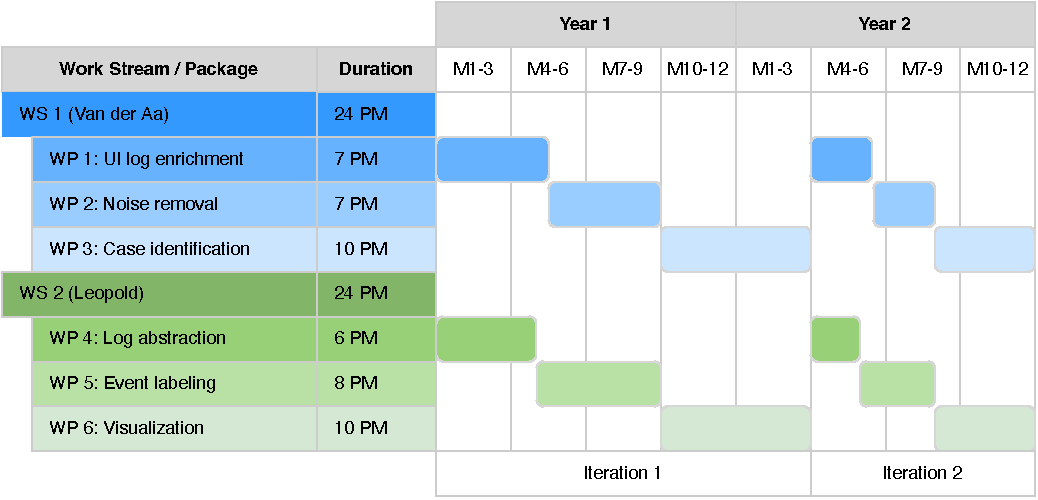
\includegraphics[width=0.8\textwidth]{./figures/Gantt.pdf}
	\caption{Work plan}
	\label{fig:workplan}
\end{figure}


As explained above, the project consists of two work streams and six work packages. 
%Naturally, there are interdependencies among these. 
\autoref{fig:workplan} shows a simplified work plan that mostly abstracts from parallel and overlapping work within each work stream. It is important to highlight that the transitions between packages will not be as strict as depicted. We are aware of the various interdependencies that exist among the packages and will take them into account appropriately.  
%There are, for instance, interdependencies between WP1 and WP2. Without an enriched UI log, the noise removal technique cannot build on the newly introduce attributes. This, however, can be addressed by taking the manually created gold standard for the evaluation of WP1 as input for WP2. In this way, the noise removal technique can already be developed without needing a ``perfect'' solution for WP1. 
The abstract view on the work plan, shown in \autoref{fig:workplan}, highlights our general idea of having two main iterations:
\begin{itemize}
	\item The first iteration ends after 15 months. At the end of this iteration, there will be a first implemented prototype available for the proposed end-to-end pipeline. The individual approaches have been evaluated both independently and as a whole. The main outcome from this iteration, therefore, are insights into the strengths and weaknesses of our work, which allows us to determine the required improvements and adaptations for the second iteration. 
	\item The second iteration is slightly shorter and will be mainly used to address identified weaknesses and improve the quality and broaden the scope of the developed approaches.
\end{itemize} 

Note that these two iterations help us to account for the aforementioned interdependencies between the work streams. In the first iteration, WS2 will build on manually refined, publicly available UI logs\footnote{\url{https://figshare.com/articles/dataset/UI_logs/12543587/4}}, while in the second iteration WS2 can use UI logs that stem from the approaches developed in WS1.  

\subsection{Handling of research data}

As explained above, we may create new synthetic UI log data sets in order to evaluate our approaches. Such data sets are not only relevant for this project, but also for other researchers in the area of process mining. In fact, the large interest in event logs has led to the creation of a central event log repository\footnote{\url{https://www.tf-pm.org/resources/logs}}, which is hosted and managed by the IEEE Task Force on Process Mining. As members of the IEEE Task Force on Process Mining, we therefore plan to make our data sets publicly available via this repository.


\subsection{Relevance of sex, gender and/or diversity}

Neither sex, gender, nor diversity will play a role in the context of this research. 